\documentclass[hidelinks, 11pt, fleqn]{article}   	% use "amsart" instead of "article" for AMSLaTeX format
\usepackage{geometry}                		% See geometry.pdf to learn the layout options. There are lots.
\usepackage{wrapfig}
\usepackage{tikz}
\usetikzlibrary{decorations.pathreplacing}
\usetikzlibrary{calc}
\usepackage{listings}
\usepackage{color}
\usepackage{amsmath}
\usepackage{mathtools}
\usepackage{algorithm}
\usepackage{algpseudocode}
\geometry{letterpaper}
\usepackage{graphicx}
\usepackage{subcaption}
\usepackage{hyperref}
\usepackage{amssymb}

\definecolor{codegreen}{rgb}{0,0.6,0}
\definecolor{codegray}{rgb}{0.5,0.5,0.5}
\definecolor{lightgray}{rgb}{0.7,0.7,0.7}
\definecolor{codepurple}{rgb}{0.58,0,0.82}
\definecolor{backcolour}{rgb}{0.92,0.92,0.92}

\renewcommand{\lstlistingname}{Algorithm}% Listing -> Algorithm

\lstdefinestyle{mystyle}{
	backgroundcolor=\color{backcolour},   
	commentstyle=\color{codegray},
	keywordstyle=\color{red},
	numberstyle=\tiny\color{lightgray},
	stringstyle=\color{codepurple},
	basicstyle=\footnotesize,
	breakatwhitespace=false,         
	breaklines=true,                 
	captionpos=b,                    
	keepspaces=true,                 
	numbers=left,                    
	numbersep=5pt,                  
	showspaces=false,                
	showstringspaces=false,
	showtabs=false,                  
	tabsize=4
}

\lstset{style=mystyle}



%SetDrawFunctions

\newcommand{\hole}[3] % x in cm, y in cm, radius in mm
{ 
	% draw hole
	\draw (#1,#2) circle (#3mm);
	% crosshair
	\draw (#1,#2-0.05) -- (#1,#2+0.05);
	\draw (#1-0.05,#2) -- (#1+0.05,#2);
	% centering lines
	\draw (#1,#2-0.1*#3-0.05) -- (#1,#2-0.1);
	\draw (#1,#2+0.1) -- (#1,#2+0.1*#3+0.05);
	\draw (#1-0.1*#3-0.05,#2) -- (#1-0.1,#2);
	\draw (#1+0.1,#2) -- (#1+0.1*#3+0.05,#2);
}
\newcommand{\dimsv}[4] % start, end, x, scale [1:x]
{
	\draw (#3-0.2,#1) -- (#3+0.2,#1);
	\draw[<-] (#3,#1) -- (#3,{(#1+#2)/2-0.2});
	\draw (#3,{(#1+#2)/2}) node {\footnotesize \pgfmathparse{(#2 - #1)*10/#4} \pgfmathprintnumber{\pgfmathresult} };
	\draw[->] (#3,{(#1+#2)/2+0.2}) -- (#3,#2);
	\draw (#3-0.2,#2) -- (#3+0.2,#2);
}
\newcommand{\dimsh}[4] % start, end, y, scale [1:x]
{
	\draw (#1,#3-0.1) -- (#1,#3+0.1);
	\draw[<-] (#1,#3) -- ({(#1+#2)/2-0.3},#3);
	\draw ({(#1+#2)/2},#3) node {\footnotesize \pgfmathparse{(#2 - #1)*10/#4} \pgfmathprintnumber{\pgfmathresult} };
	\draw[->] ({(#1+#2)/2+0.3},#3) -- (#2,#3);
	\draw (#2,#3-0.1) -- (#2,#3+0.1);
}

%SetFonts
\newtagform{brackets}{[}{]}
\usetagform{brackets}

\title{\textbf{CNC Router}}
\author{Patrick Sorn}

\begin{document}
\maketitle
\tableofcontents 
\pagebreak
\section{Introduction}
\pagebreak
\section{Portal}
\subsection{Base Plate}

\begin{figure}[h]
	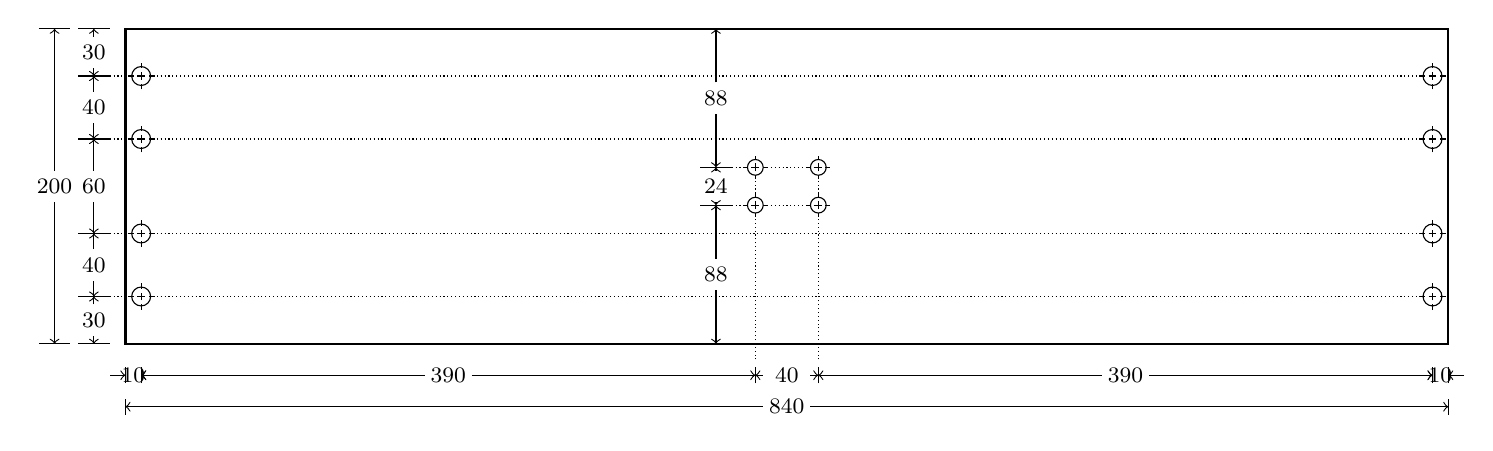
\begin{tikzpicture}
	% 84cm x 20cm x 12mm
	% scale 1:5
	\draw[thick] (0, 0) rectangle (16.8, 4.0);
	\hole{0.2}{0.6}{1.2};
	\hole{0.2}{1.4}{1.2};
	\hole{0.2}{2.6}{1.2};
	\hole{0.2}{3.4}{1.2};
	
	\hole{16.6}{0.6}{1.2};
	\hole{16.6}{1.4}{1.2};
	\hole{16.6}{2.6}{1.2};
	\hole{16.6}{3.4}{1.2};
	
	\hole{8}{1.76}{1};
	\hole{8}{2.24}{1};
	\hole{8.8}{1.76}{1};
	\hole{8.8}{2.24}{1};
	
	\dimsh{0}{0.2}{-0.4}{0.2};
	\dimsh{0.2}{8}{-0.4}{0.2};
	\dimsh{8}{8.8}{-0.4}{0.2};
	\dimsh{8.8}{16.6}{-0.4}{0.2};
	\dimsh{16.6}{16.8}{-0.4}{0.2};
	\dimsh{0}{16.8}{-0.8}{0.2};
	
	\draw[densely dotted] (8, -0.2) -- (8, 1.66);
	\draw[densely dotted] (8, 1.86) -- (8, 2.14);
	\draw[densely dotted] (8.8, -0.2) -- (8.8, 1.66);
	\draw[densely dotted] (8.8, 1.86) -- (8.8, 2.14);
	
	\dimsv{0}{0.6}{-0.4}{0.2};
	\dimsv{0.6}{1.4}{-0.4}{0.2};
	\dimsv{1.4}{2.6}{-0.4}{0.2};
	\dimsv{2.6}{3.4}{-0.4}{0.2};
	\dimsv{3.4}{4.0}{-0.4}{0.2};
	\dimsv{0}{4.0}{-0.9}{0.2};
	
	\draw[densely dotted] (-0.2, 0.6) -- (0.1, 0.6);
	\draw[densely dotted] (0.3, 0.6) -- (16.5, 0.6);
	\draw[densely dotted] (-0.2, 1.4) -- (0.1, 1.4);
	\draw[densely dotted] (0.3, 1.4) -- (16.5, 1.4);
	\draw[densely dotted] (-0.2, 2.6) -- (0.1, 2.6);
	\draw[densely dotted] (0.3, 2.6) -- (16.5, 2.6);
	\draw[densely dotted] (-0.2, 3.4) -- (0.1, 3.4);
	\draw[densely dotted] (0.3, 3.4) -- (16.5, 3.4);
	
	\dimsv{0}{1.76}{7.5}{0.2};
	\dimsv{1.76}{2.24}{7.5}{0.2};
	\dimsv{2.24}{4.0}{7.5}{0.2};
	
	\draw[densely dotted] (7.7, 1.76) -- (7.9, 1.76);
	\draw[densely dotted] (8.1, 1.76) -- (8.9, 1.76);
	\draw[densely dotted] (7.7, 2.24) -- (7.9, 2.24);
	\draw[densely dotted] (8.1, 2.24) -- (8.9, 2.24);

	\end{tikzpicture}
\caption{Base Plate.}
\label{fig:base_plate}
\end{figure}

\subsection{Side Plate}

\begin{figure}[h]
	\begin{tikzpicture}
	% 20cm x 40cm x 20mm
	% scale 1:2
	%\draw[thick] (0, 0) rectangle (10, 20);
	\draw[thick] (0, 0) -- (10, 0) -- (10, 20) -- (5, 20) -- (0, 10) -- (0, 0);
	\draw[dotted] (0, 10) -- (0, 20) -- (5, 20);
	\hole{0.6}{2.2}{1.5};
	\hole{0.6}{3.95}{1.5};
	\hole{2.35}{2.2}{1.5};
	\hole{2.35}{3.95}{1.5};
	
	\hole{7.65}{2.2}{1.5};
	\hole{7.65}{3.95}{1.5};
	\hole{9.4}{2.2}{1.5};
	\hole{9.4}{3.95}{1.5};
	
	\hole{9.25}{11.75}{2};
	\hole{9.25}{19.25}{2};
	
	\hole{6.85}{14.3}{1};
	\hole{6.85}{16.65}{1};
	\hole{9.2}{14.3}{1};
	\hole{9.2}{16.65}{1};
	
	\hole{8.025}{15.475}{6.5};
	
	
	\dimsh{0}{0.6}{-0.3}{0.5};
	\dimsh{0.6}{2.35}{-0.3}{0.5};
	\dimsh{2.35}{7.65}{-0.3}{0.5};
	\dimsh{7.65}{9.4}{-0.3}{0.5};
	\dimsh{9.4}{10}{-0.3}{0.5};
	\dimsh{0}{10}{-0.7}{0.5};
	
	\draw[densely dotted] (0.6, -0.2) -- (0.6, 2.1);
	\draw[densely dotted] (0.6, 2.3) -- (0.6, 3.85);
	\draw[densely dotted] (2.35, -0.2) -- (2.35, 2.1);
	\draw[densely dotted] (2.35, 2.3) -- (2.35, 3.85);
	\draw[densely dotted] (7.65, -0.2) -- (7.65, 2.1);
	\draw[densely dotted] (7.65, 2.3) -- (7.65, 3.85);
	\draw[densely dotted] (9.4, -0.2) -- (9.4, 2.1);
	\draw[densely dotted] (9.4, 2.3) -- (9.4, 3.85);
	
	\dimsv{0}{2.2}{10.4}{0.5};
	\dimsv{2.2}{3.95}{10.4}{0.5};
	\dimsv{3.95}{11.75}{10.4}{0.5};
	\dimsv{11.75}{14.3}{10.4}{0.5};
	\dimsv{14.3}{16.65}{10.4}{0.5};
	\dimsv{16.65}{19.25}{10.4}{0.5};
	\dimsv{19.25}{20}{10.4}{0.5};
	\dimsv{0}{20}{10.9}{0.5};
	
	\draw[densely dotted] (0.7, 2.2) -- (2.25, 2.2);
	\draw[densely dotted] (2.45, 2.2) -- (7.55, 2.2);
	\draw[densely dotted] (7.75, 2.2) -- (9.3, 2.2);
	\draw[densely dotted] (9.5, 2.2) -- (10.2, 2.2);
	\draw[densely dotted] (0.7, 3.95) -- (2.25, 3.95);
	\draw[densely dotted] (2.45, 3.95) -- (7.55, 3.95);
	\draw[densely dotted] (7.75, 3.95) -- (9.3, 3.95);
	\draw[densely dotted] (9.5, 3.95) -- (10.2, 3.95);
	
	\draw[densely dotted] (9.35, 11.75) -- (10.2, 11.75);
	\draw[densely dotted] (9.35, 19.25) -- (10.2, 19.25);
	
	\dimsh{0}{9.25}{11.35}{0.5};
	\dimsh{9.25}{10}{11.35}{0.5};
	
	\draw[densely dotted] (9.25, 11.85) -- (9.25, 19.15);
	
	\draw[densely dotted] (7, 14.3) -- (9.15, 14.3);
	\draw[densely dotted] (9.35, 14.3) -- (10.2, 14.3);
	\draw[densely dotted] (7, 16.65) -- (9.15, 16.65);
	\draw[densely dotted] (9.35, 16.65) -- (10.2, 16.65);
	
	\dimsh{0}{6.85}{13.9}{0.5};
	\dimsh{6.85}{9.2}{13.9}{0.5};
	\dimsh{9.2}{10}{13.9}{0.5};
	
	\draw[densely dotted] (6.85, 14) -- (6.85, 14.2);
	\draw[densely dotted] (6.85, 14.4) -- (6.85, 16.55);
	\draw[densely dotted] (9.2, 14) -- (9.2, 14.2);
	\draw[densely dotted] (9.2, 14.4) -- (9.2, 16.55);
	
	
	
	\end{tikzpicture}
\caption{Side Plate.}
\label{fig:side_plate}
\end{figure}

\end{document}